\section{Lifting line theory summary}
This section summarizes the main ideas and equations of lifting line theory:

\subsection{Lift of an airfoil}
The lift produced by an infinitesimal span airfoil $L_y$ in steady state is given by the Kutta–Joukowski theorem: 
\begin{equation}
    \frac{dL}{dy} = L_y = \rho V \Gamma(y, \alpha)
\end{equation}

Where $\Gamma$ represents the circulation around the airfoil. If the airfoil is at an angle $\alpha$, the lift is given by \cite[eqn 21]{leishman}:
\begin{equation}
    \Gamma = \frac{V}{2} c(y) c_l(\alpha(y)) \approx \frac{V}{2} c(y) \left(2 \pi (\alpha(y)\right)
\end{equation}
Where $c(y)$ is the local chord length and $\alpha(y)$ is the local angle of attack considering any wing twist.

The lift can be integrated over the span to obtain the total lift.

\subsection{Lifiting line}
Because the circulation is not constant along the wingspan, the variation in circulation needs to be compensated by the shedding of a vortex. The shed vortices instead induce a vertical velocity over the wingspan.

This induced velocity can be computed by:
\begin{equation}
    w(y) = \int_{-b/2}^{b/2} \frac{d\Gamma(\tilde{y})}{4\pi\left(y - \tilde{y}\right)}
\end{equation}

Note the integrand is singular at $y = \tilde{y}$, so it is understood in terms of the Cauchy principal value.

The circulation at a point can be extended to account for the effect of the induced velocity:
\begin{align}
    \Gamma(y)   &= \frac{V}{2} c(y)  c_l\left( \alpha(y) + \frac{w(y)}{V}\right) \\
                &\approx \frac{V}{2} c(y) 2 \pi\left(\alpha(y) + \frac{1}{V} \int_{-b/2}^{b/2} \frac{d\Gamma(\tilde{y})}{4\pi\left(y - \tilde{y}\right)} \right)
\end{align}

And the total lift and drag can be computed as \cite[eqn 22]{leishman}:
\begin{align}
    L &= \rho V  \int_{-b/2}^{b/2} \Gamma(y, \alpha) dy \\
    D &= \rho V \int_{-b/2}^{b/2} \Gamma(y, \alpha) \frac{w(y)}{V} dy
\end{align}

Note: wikipedia states the induced drag includes $\alpha(y)$ instead of $w(y)$, however this could lead to induced drag simply due to the angle of attack in the case of an infinite wing.

\section{Solution}
The solution process consists of find the circulation profile for a given wing geometry, i.e. $c(y)$ and $\alpha(y)$.

In order to compute the circulation profile, we can discretize the problem and solve it numerically.

\subsection{Discretization scheme}
Since we are considering an integral in the Cauchy singular value sense, we will discretize the integral using a rectangle rule.

The rectangle rule value is done as follows:
\begin{equation}
    F(x) = \int_{a}^{b} f(x) dx \approx \sum_{i=0}^{N} f(x_i) \Delta x_i
\end{equation}

Where $\Delta$ is the difference operator which can be expressed as:
\begin{equation}
    \Delta f(x_i) = \frac{f(x_{i+1}) - f(x_{i-1})}{2}
\end{equation}

Considering that at the limits we will instead use:
\begin{align}
    \Delta f(x_0) &= \frac{f(x_1) - f(x_0)}{2} \\
    \Delta f(x_N) &= \frac{f(x_N) - f(x_{N-1})}{2}
\end{align}

This rule let us compute the Cauchy value by simply excluding the integrand at the singularity point.

\subsubsection{Difference operator as a toeplitz matrix}
The difference operator can be implemnted using an modified toeplitz matrix that works as an operator on a vector:

\begin{equation}
    \Delta x = 
    \begin{bmatrix}
        -1/2 & +1/2 & 0 & 0 &\cdots & 0 & 0 & 0 & 0\\
        -1/2 & 0 & +1/2 & 0 & \cdots & 0 & 0 & 0 & 0\\
        0 &-1/2 & 0 & +1/2 & \cdots & 0 & 0 & 0 & 0\\
        \vdots & \vdots & \vdots & \vdots & \ddots & \vdots & \vdots & \vdots & \vdots \\
        0 & 0 & 0 & 0 & \cdots & -1/2 & 0 & +1/2 & 0 \\
        0 & 0 & 0 & 0 & \cdots & 0 & -1/2 & 0 & +1/2 \\
        0 & 0 & 0 & 0 & \cdots & 0 & 0 & -1/2 & +1/2 \\
    \end{bmatrix}
    \begin{bmatrix}
        x_0 \\
        x_1 \\
        x_2 \\
        \vdots \\
        x_{N-2} \\
        x_{N-1} \\
        x_N
    \end{bmatrix}
\end{equation}

So $\Delta$ can be readily handled as a matrix.

\subsubsection{Example of the integration of a Cauchy singular value}
We could check the accuracy of this scheme by integrating:
\begin{equation}
    F(x) = \int_{-1}^{2}\frac{dx}{x}
\end{equation}

The function is odd about the singularity at $x=0$, which is the use case for the Cauchy singular value, so we can split the integration into two parts and play with the limits.
Whose analytic solution is:
\begin{align}
    F(x)    &= \int_{-1}^{-\epsilon} \frac{dx}{x} + \int_{\epsilon}^{2} \frac{dx}{x} = \\
            &= \int_{1}^{\epsilon} \frac{dx}{x} + \int_{\epsilon}^{2} \frac{dx}{x} = \\
            &= \left. \ln(x) \right|_{1}^{\epsilon} + \left. \ln(x) \right|_{\epsilon}^{2} = \\
            &= \ln(2) - \ln(1) = \ln (2)
\end{align}

This problem is solved in \texttt{midpoint\_test.py} as a test for the integration scheme.

\subsection{Discretization of the circulation}
We can discretize the problem.
\begin{equation}
    \Gamma(y_i) = \frac{V}{2} c(y_i) 2 \pi \left( \alpha(y_i) + \frac{1}{4\pi V}\sum_{j=1}^{N} \frac{\Delta\Gamma(y_j)}{\left(y_i - y_j\right)} \right)
\end{equation}

Where $\Delta$ is the difference operator defined above.

\subsubsection{Expression as a matrix}
The expression above can be more clearly stated in a matrix form using the notation $f_i$ to denote the value of $f(y_i)$:
\begin{equation}
    \Gamma_i = \frac{V}{2} c_i 2 \pi \left( \alpha_i + \frac{1}{4\pi V}\sum_{j=1}^{N} \frac{\Delta\Gamma_j}{\left(y_i - y_j\right)} \right)
\end{equation}

We realize that the the sum over $j$ can be expressed as a matrix product since:
\begin{equation}
    c_i = \sum_{j=1}^{N} A_{ij}b_j
\end{equation}

We will denote with $\left[A_{ij}\right]_{ij}$ the matrix with the elements $A_{ij}$ in the position $(i,j)$. Any undefined elements are understood to be zero.

The result is:
\begin{equation}
    \Gamma= \frac{V}{2} \left[c_i\right]_{ii} 2 \pi \left( \alpha + \frac{1}{4\pi V} \left[\frac{1}{\left(y_i - y_j\right)}\right]_{ij,i\neq j}\Delta\Gamma \right)
\end{equation}

The matrix $\left[\frac{1}{\left(y_i - y_j\right)}\right]_{ij}$ would have singular values for $i=j$ so these values are left undefined so they are zeroed, this consider the Cauchy principal value. Similarly, $\left[c_i\right]_{ii}$ denotes a diagonal matrix with $c_i$ as the diagonal elements.

After all this, solving for  $\Gamma$ is simple matrix manipulation:
\begin{equation}
    \Gamma = \left(I- \frac{V}{2} \left[c_i\right]_{ii} 2 \pi \frac{1}{4\pi V} \left[\frac{1}{\left(y_i - y_j\right)}\right]_{ij,i\neq j}\Delta \right)^{-1} \frac{V}{2} D(c) 2 \pi \alpha
\end{equation}

\subsection{Example solution}
We consider the solution here for a large solar aircraft with similar characteristics to Skydweller.

We compute the lift and drag distribution and we compare it the ideal lift distribution:

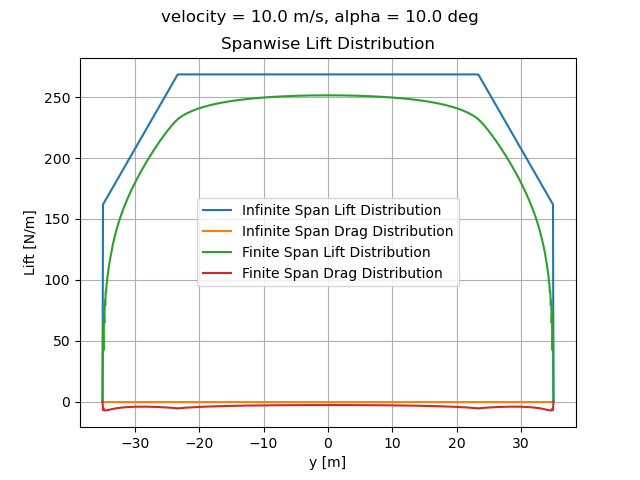
\includegraphics[width=\textwidth]{input/ex_lift_drag_distribution.png}

And the distribution of induced angles of attacks is:

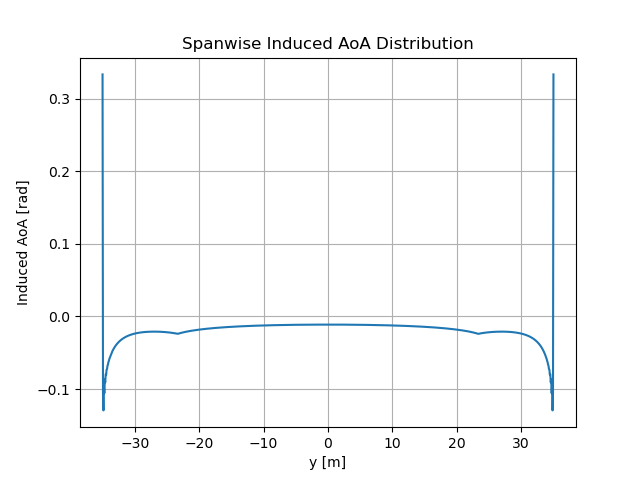
\includegraphics[width=\textwidth]{input/ex_induced_alpha.png}

\def\lift{15685.37}
\def\drag{276.02}
\def\clalpha{5.61}
\def\lifttodrag{56.83}
\def\efficiency{0.90}
\def\clalphatheory{5.62}
\def\lifttodragtheory{54.07}


The lift coefficient $C_{L_\alpha}$ produced by the finite wing is \clalpha{} \. The induced drag is produced mainly close to the wingtips where the vortex intensity is higher and modifies the apparent angle of attack. The observed lift to induced drag ratio is \lifttodrag{}.

\subsection{Comparison with theoretical values}
In this section we compare the results above with the theoretical values of the lift coefficient and drag coefficients.

The finite wing $C_{L_\alpha}$ is given by \cite[eqn 73]{leishman}:
\begin{equation}
    C_{L_\alpha}= \frac{C_{L_{\alpha_\infty}}}{1 + \dfrac{C_{L_{\alpha_\infty}}}{\pi e \Lambda}}
\end{equation}

Where $\Lambda$ is the aspect ratio, and $e$ is the Oswald efficiency factor, which is 1 for an elliptical wing. Assuming an Oswald efficiency factir of \efficiency{}, the resulting theoretical $C_{L_\alpha}$ is \clalphatheory{}, quite close to \clalpha{}.

The induced drag is given by \cite[eqn 49]{leishman}:
\begin{equation}
    C_{D_{i}} = \frac{C_L^2}{\pi e \Lambda}
\end{equation}

The theoretical aerodynamics efficiency is \lifttodragtheory{}, similar to the previously obtained \lifttodrag{}.

\printbibliography[title={References}]